% Première ligne : Sigmoïde & Tanh
\begin{minipage}{0.45\textwidth}
\centering
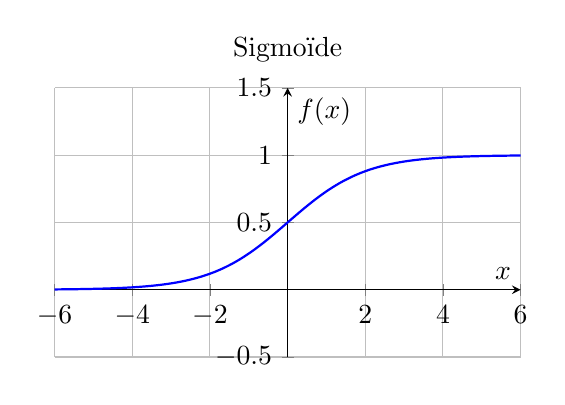
\begin{tikzpicture}
\begin{axis}[
    width=7.5cm,
    height=5cm,
    title={Sigmoïde},
    axis lines=middle,
    xlabel={$x$},
    ylabel={$f(x)$},
    xmin=-6, xmax=6,
    ymin=-0.5, ymax=1.5,
    samples=200,
    domain=-6:6,
    grid=both
]
\addplot[blue, thick] {1 / (1 + exp(-x))};
\end{axis}
\end{tikzpicture}
\end{minipage}
\hfill
\begin{minipage}{0.45\textwidth}
\centering
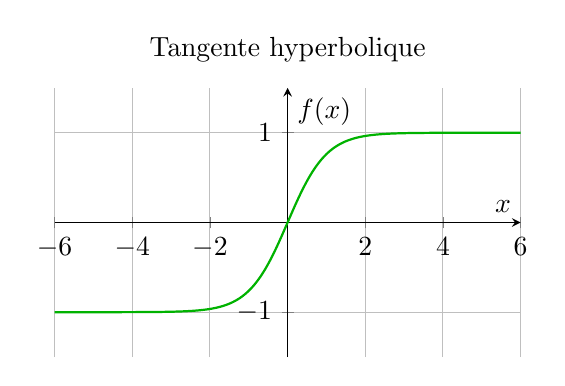
\begin{tikzpicture}
\begin{axis}[
    width=7.5cm,
    height=5cm,
    title={Tangente hyperbolique},
    axis lines=middle,
    xlabel={$x$},
    ylabel={$f(x)$},
    xmin=-6, xmax=6,
    ymin=-1.5, ymax=1.5,
    samples=200,
    domain=-6:6,
    grid=both
]
\addplot[green!70!black, thick] {tanh(x)};
\end{axis}
\end{tikzpicture}
\end{minipage}

\vspace{0.1cm}

% Deuxième ligne : ReLU & Softplus
\begin{minipage}{0.45\textwidth}
\centering
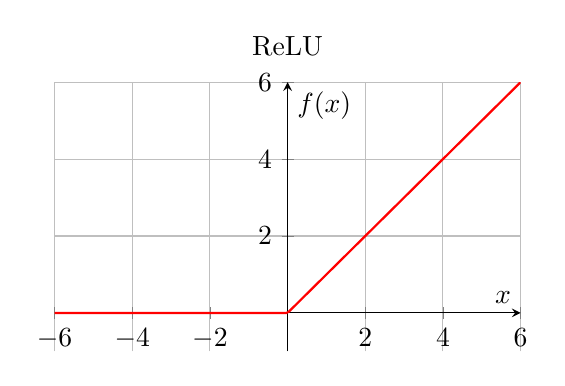
\begin{tikzpicture}
\begin{axis}[
    width=7.5cm,
    height=5cm,
    title={ReLU},
    axis lines=middle,
    xlabel={$x$},
    ylabel={$f(x)$},
    xmin=-6, xmax=6,
    ymin=-1, ymax=6,
    samples=200,
    domain=-6:6,
    grid=both
]
\addplot[red, thick] {max(0, x)};
\end{axis}
\end{tikzpicture}
\end{minipage}
\hfill
\begin{minipage}{0.45\textwidth}
\centering
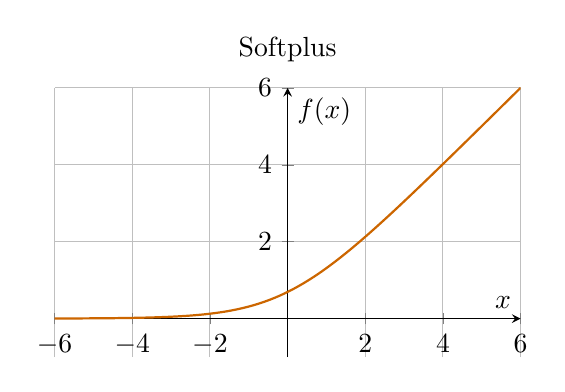
\begin{tikzpicture}
\begin{axis}[
    width=7.5cm,
    height=5cm,
    title={Softplus},
    axis lines=middle,
    xlabel={$x$},
    ylabel={$f(x)$},
    xmin=-6, xmax=6,
    ymin=-1, ymax=6,
    samples=200,
    domain=-6:6,
    grid=both
]
\addplot[orange!80!black, thick] {ln(1 + exp(x))};
\end{axis}
\end{tikzpicture}
\end{minipage}

\vspace{0.2cm}

% LIGNE 3 : Heaviside & Leaky ReLU
\begin{minipage}{0.45\textwidth}
\centering
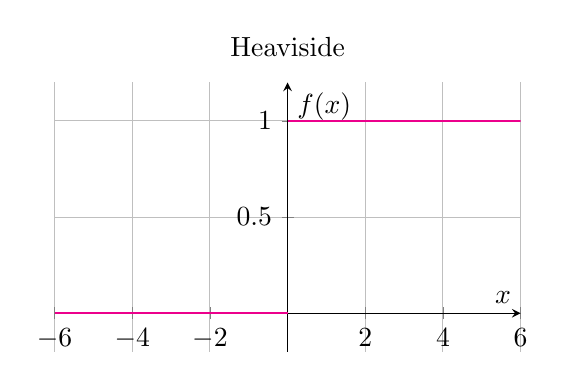
\begin{tikzpicture}
\begin{axis}[
    width=7.5cm, height=5cm,
    title={Heaviside},
    axis lines=middle,
    xlabel={$x$}, ylabel={$f(x)$},
    xmin=-6, xmax=6, ymin=-0.2, ymax=1.2,
    samples=2, domain=-6:6,
    grid=both]
\addplot[magenta, thick, domain=-6:0] {0};
\addplot[magenta, thick, domain=0.01:6] {1};
\end{axis}
\end{tikzpicture}
\end{minipage}
\hfill
\begin{minipage}{0.45\textwidth}
\centering
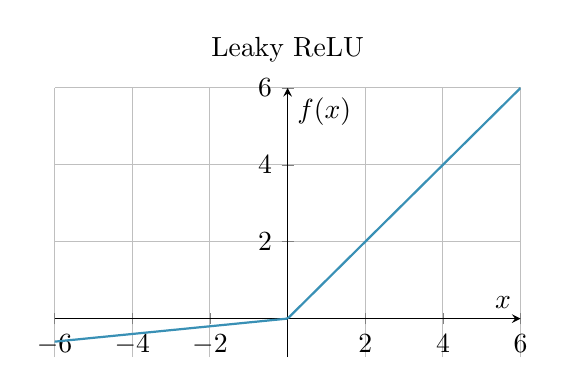
\begin{tikzpicture}
\begin{axis}[
    width=7.5cm, height=5cm,
    title={Leaky ReLU},
    axis lines=middle,
    xlabel={$x$}, ylabel={$f(x)$},
    xmin=-6, xmax=6, ymin=-1, ymax=6,
    samples=200, domain=-6:6,
    grid=both]
\addplot[cyan!70!black, thick, domain=-6:6] { (x < 0) * 0.1 * x + (x >= 0) * x };
\end{axis}
\end{tikzpicture}
\end{minipage}

